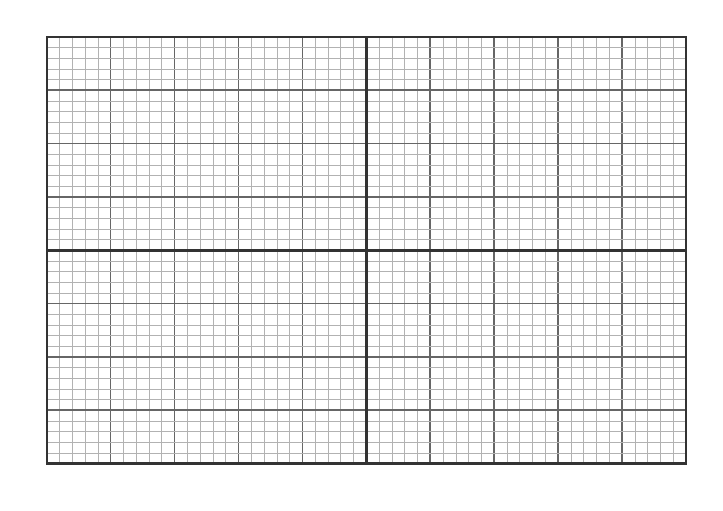
\begin{tikzpicture}
    \begin{axis}[
        width=0.8\textwidth,
        height=7cm,
        grid=both,
        major grid style={line width=.6pt,draw=black!60},
        minor grid style={line width=.2pt,draw=black!30},
        xmin=0, xmax=10,
        ymin=-4, ymax=4,
        xtick={0,1,2,3,4,5,6,7,8,9,10},
        ytick={-4,-3,-2,-1,0,1,2,3,4},
        minor x tick num=4,
        minor y tick num=4,
        xticklabels={},
        yticklabels={},
        tick style={draw=none},
        axis line style={draw=black!80, thick},
    ]
        % Ejes centrales más marcados
        \draw[line width=1pt, black!80] (axis cs:0,0) -- (axis cs:10,0);
        \draw[line width=1pt, black!80] (axis cs:5,-4) -- (axis cs:5,4);
    \end{axis}
\end{tikzpicture}
